\documentclass[11pt]{article}

\usepackage[top=1in,bottom=1.25in,left=1.25in,right=1.25in]{geometry}

\usepackage{graphicx}
\usepackage{ragged2e}
\usepackage{tabto}
\usepackage{amssymb}
\usepackage{float}
\usepackage{amsmath}
\usepackage{multirow}
\usepackage{amsthm}
\usepackage{epsfig}
\usepackage{subfigure}
\usepackage{amscd}
\usepackage{color}
\usepackage{url}
\usepackage{hyperref}
\usepackage{cleveref}

\usepackage{afterpage}
\usepackage{fancybox}
\usepackage{ifthen}
\usepackage{multicol}
\usepackage[font=footnotesize]{caption}


\usepackage{lmodern}
%\usepackage{newtxtext}
%\usepackage{newtxmath}https://www.overleaf.com/project/5e8260a3d5a8e1000145aa85
\usepackage{siunitx}
\sisetup{range-phrase=--, fixed-exponent=2, range-units =single, table-number-alignment =center, table-figures-exponent=1}
\usepackage[sf,bf,medium]{titlesec}

%\usepackage{bm}
\usepackage{dsfont}
\usepackage{booktabs}
%\usepackage{isomath}
%\newcommand{\vct}{\vectorsym}
%\newcommand{\mtx}{\matrixsym}


\newcommand\dbarb{\bar{\partial}_b}
\newcommand\boxb{\square_b}
\DeclareMathOperator\eo{eo}
\DeclareMathOperator\ooee{oe}
%\newcommand\comp{\operatorname{comp}}
\newcommand\w{\wedge}
\newcommand{\todo}[1]{{\color{red}#1}}
\newcommand\dx{\dot{x}}
\newcommand\dz{\dot{z}}
\newcommand\dVol{\operatorname{dV}}
\newcommand\lot{\operatorname{l.o.t.}}
\newcommand\Reg{\operatorname{Reg}}
\newcommand\dom{\operatorname{Dom}}
\newcommand\diag{\operatorname{diag}}
\newcommand\loc{\operatorname{loc}}
\newcommand\Dom{\operatorname{Dom}}
\newcommand\Dir{\operatorname{Dir}}
\newcommand\Def{\operatorname{Def}}
\newcommand\cdeg{\operatorname{c-deg}}
\newcommand\sing{\operatorname{Sing}}
\newcommand\sign{\operatorname{sig}}
\newcommand\SW{\operatorname{SW}}
\newcommand\dist{\operatorname{dist}}
\newcommand\eucl{\operatorname{eucl}}
\newcommand\relp{\operatorname{P}}
\newcommand\Span{\operatorname{span}}
\newcommand\tot{\operatorname{tot}}
\newcommand\In{\operatorname{in}}
\newcommand\scat{\operatorname{scat}}
\newcommand\Int{\operatorname{int}}
\newcommand\hone{h^{(1)}}
\newcommand\out{\operatorname{out}}
\newcommand\spnc{\operatorname{Spin}_{\bbC}}
\newcommand\Th{\operatorname{th}}
\newcommand\Tr{\operatorname{tr}}
\newcommand\iso{\operatorname{iso}}
\newcommand\Spec{\operatorname{spec}}
\newcommand\hn{(1,-\frac 12)}
\newcommand\cT{\mathcal T}
\newcommand\cM{\mathcal M}
\newcommand\cN{\mathcal N}
\newcommand\cH{\mathcal H}
\newcommand\cI{\mathcal I}
\newcommand\cJ{\mathcal J}
\newcommand\cO{\mathcal O}
\newcommand\cU{\mathcal U}
\newcommand\cV{\mathcal V}
\newcommand\sO{\mathfrak O}
\newcommand\fT{\mathfrak T}
\newcommand\cQ{\mathcal Q}
\newcommand\cK{\mathcal K}
\newcommand\cG{\mathcal G}
\newcommand\cB{\mathcal B}
\newcommand\cR{\mathcal R}
\newcommand\cP{\mathcal P}
\newcommand{\ccD}{\mathfrak D}
\newcommand\ho{\mathfrak H}
\newcommand\px{\tilde x}
\newcommand\pz{\tilde z}
\newcommand\bc{\boldsymbol c}
\newcommand\bb{\boldsymbol b}
\newcommand\ba{\boldsymbol a}
\newcommand\bzero{\boldsymbol 0}
\newcommand\balpha{\boldsymbol \alpha}
\newcommand\bgamma{\boldsymbol \gamma}
\newcommand\btheta{\boldsymbol \theta}
\newcommand\bpsi{\overline{\psi}}
\newcommand\bEta{\boldsymbol \eta}
\newcommand\tbEta{\widetilde{\boldsymbol \eta}}
\newcommand\tbB{\widetilde{\boldsymbol B}}
\newcommand\bBeta{\boldsymbol \beta}
\newcommand\bj{\boldsymbol j}
\newcommand\bl{\boldsymbol l}
\newcommand\tj{\widetilde j}
\newcommand\tphi{\widetilde \phi}
\newcommand\tpsi{\widetilde \psi}
\newcommand\tk{\tilde k}
\newcommand\tu{\widetilde u}
\newcommand\tv{\widetilde v}
\newcommand\tD{\widetilde D}
\newcommand\tM{\widetilde M}
\newcommand\tN{\widetilde N}
\newcommand\tP{\widetilde P}
\newcommand\tL{\widetilde L}
\newcommand\hdy{\widehat{dy}}
\newcommand\hdx{\widehat{dx}}
%%\newcommand\bk{\boldsymbol k}
\newcommand\bm{\boldsymbol m}
\newcommand\bK{\boldsymbol K}
\newcommand\bv{\boldsymbol v}
\newcommand\bn{\boldsymbol n}
\newcommand\br{\boldsymbol r}
\newcommand\tbn{\boldsymbol {\tilde{n}}}
\newcommand\bq{\boldsymbol q}
\newcommand\bx{\boldsymbol x}
\newcommand\by{\boldsymbol y}
\newcommand\hbx{\hat{\boldsymbol x}}
\newcommand\bA{\boldsymbol A}
\newcommand\bB{\boldsymbol B}
\newcommand\bD{\boldsymbol D}
\newcommand\bH{\boldsymbol H}
\newcommand\bL{\boldsymbol L}
\newcommand\bE{\boldsymbol E}
\newcommand\bV{\boldsymbol V}
\newcommand\bJ{\boldsymbol J}
\newcommand\bN{\boldsymbol N}
\newcommand\bP{\boldsymbol P}
\newcommand\bR{\boldsymbol R}
\newcommand\bX{\boldsymbol X}
\newcommand\bY{\boldsymbol Y}
\newcommand\bPhi{\boldsymbol \Phi}
\newcommand\bPsi{\boldsymbol \Psi}

\newcommand\bT{\boldsymbol T}
\newcommand\fS{\mathfrak S}
\newcommand\bcP{\bar{\cP}}
\newcommand\tcP{\widetilde{\cP}}
\newcommand\cF{\mathcal F}
\newcommand\cE{\mathcal E}
\newcommand\cW{\mathcal W}
\newcommand\bS{\bar{S}}
\newcommand\bF{\bar{F}}
\newcommand\bcF{\bar{\cF}}
\newcommand\dbar{\bar{\pa}}
\newcommand\dbnc{\dbar\rho\rfloor}
\newcommand\tnabla{\widetilde{\nabla}}
\newcommand\bz{\bar{z}}
\newcommand\sypr{\pi}
\newcommand\syprc{\bar{\pi}}
\newcommand\scp{\mathfrak p}
\newcommand\sd{\mathfrak d}
\newcommand\bzeta{\bar{\zeta}}
\newcommand\bxi{\boldsymbol \xi}
\newcommand\tbxi{\widetilde{\bxi}}
\newcommand\tbE{\widetilde{\bE}}
\newcommand\tbH{\widetilde{\bH}}
\newcommand\bXi{\boldsymbol \Xi}
\newcommand\bcQ{\bar{\mathcal Q}}
\newcommand\starb{\star_b}
\newcommand\talpha{\widetilde{\alpha}}
\newcommand\tbeta{\widetilde{\beta}}
\newcommand\tgamma{\widetilde{\gamma}}
\newcommand\ta{\widetilde{a}}
\newcommand\tq{\widetilde{q}}
\newcommand\tQ{\widetilde{Q}}
\newcommand\txi{\widetilde{\xi}}
\newcommand\tOmega{\widetilde{\Omega}}
\newcommand\tX{\widetilde{X}}
\newcommand\pX{X'}
\newcommand\thX{\widetilde{\pX}}
\newcommand\hX{\widehat{X}}
\newcommand\hx{\widehat{x}}
\newcommand\hg{\widehat{g}}
\newcommand\hmu{\widehat{\mu}}
\newcommand\hD{\widehat{D}}
\newcommand\hpsi{\widehat{\psi}}
\newcommand\tK{\widetilde{K}}
\newcommand\sh[1]{\overset{\sqcap}{#1}}
\newcommand\RC[1]{{}^R\overline{T^*{#1}}}
\newcommand\HC[1]{{}^H\overline{T^*{#1}}}
\newcommand\EHC[1]{{}^{eH}\overline{T^*{#1}}}
\newcommand\sym[1]{{}^{#1}\sigma}
\newcommand\esym[2]{{}^{#1}\sigma^{#2}}
\newcommand\Tzo[1]{{}^{#1}T^{0,1}}
\newcommand\Toz[1]{{}^{#1}T^{1,0}}
\newcommand\ie{i\@.e\@.\ }
\newcommand\eg{e\@.g\@. }
\newcommand\viz{\emph{viz\@.}}
\newcommand{\Spn}{S\mspace{-10mu}/ }
\newcommand{\THME[1]}{THME(#1)}

\newcommand\CC{\hbox{\mathbb C}}
\newcommand\DD{\hbox{\mathbb D}}
\newcommand\RR{\hbox{\mathbb R}}
\newcommand\PP{\hbox{\mathbb P}}
\newcommand\bsl{\backslash}
\newcommand\ep{\varepsilon}
%\newcommand\pa{\partial}
\newcommand\vphi{\varphi}


\newcommand\Ker{\operatorname{ker}}
\newcommand\PV{\operatorname{P.V.}}
\newcommand\coker{\operatorname{coker}}
\newcommand\hotimes{\hat\otimes}
\newcommand\cA{\mathcal{A}}
\newcommand\cC{\mathcal{C}}
\newcommand\cL{\mathcal{L}}
\newcommand\cS{\mathcal{S}}
\newcommand\hcS{\widehat{\mathcal{S}}}
\newcommand\bcS{\bar{\mathcal{S}}}
\newcommand\cD{\mathcal{D}}
\newcommand\hz{\hat z}
\newcommand\hOmega{\widehat \Omega}
\newcommand\cz{\check z}
\newcommand\hal{\hat \alpha }
\newcommand\hZ{\hat Z}
\newcommand\cZ{\check Z}
\newcommand\dZ{\dot Z}
\newcommand\hu{\hat u}
\newcommand\cu{\check u}
\newcommand\hv{\hat v}
\newcommand\cv{\check v}
\newcommand\hzeta{\hat\zeta}
\newcommand\czeta{\check\zeta}
\newcommand\dzeta{\dot\zeta}
\newcommand\hsigma{\hat\sigma}
\newcommand\sigmah{\sigma^H}
\newcommand\nsigma{\sigma_\nu}
\newcommand\bsigma{\sigma_b}
\newcommand\tsigma{\tilde\sigma}
\newcommand\vol{\operatorname{vol}}
\newcommand\tf{\tilde{f}}
\newcommand\bZ{\overline{Z}}
\newcommand\Zup{\overline{\bbC_+}}
\newcommand\bW{\overline{W}}
\newcommand\bomega{\boldsymbol{\omega}}
%%%%% Some general AMSLatex macros
%\setlength{\marginparwidth}{0.72in}
%\newcommand{\mar}[1]{{\marginpar{\sffamily{\scriptsize #1}}}}
%{{\marginpar{\textsf{#1}}}}
\newcommand\datver[1]{\def\datverp%
 {\par\boxed{\boxed{\text{#1; Run: \today}}}}}
\newcommand\ha{\frac12}
\newcommand\oqu{\frac14}
\renewcommand\Re{\operatorname{Re}}
\renewcommand\Im{\operatorname{Im}}
\newcommand\fiber{\operatorname{fiber}}
\newcommand\fdim{\operatorname{fiber-dim}}
\newcommand\fa{\mathfrak a}
\newcommand\fb{\mathfrak b}
\newcommand\fc{\mathfrak c}
\newcommand\CAS{\mathcal{S}}
\newcommand\CAFS{\mathcal{FS}}
\newcommand\CAJ{\mathcal{J}}
\newcommand\bbB{\mathbb B}
\newcommand\bbC{\mathbb C}
\newcommand\bbD{\mathbb D}
\newcommand\bbH{\mathbb H}
\newcommand\bbQ{\mathbb Q}
\newcommand\bbN{\mathbb N}
\newcommand\bbP{\mathbb P}
\newcommand\bbR{\mathbb R}
\newcommand\bbZ{\mathbb Z}
\newcommand\bbS{\mathbb S}
\newcommand\bbT{\mathbb T}
\newcommand\Npat{N_{\textrm{patches}}}
\newcommand\smax{s_{\textrm{max}}}
\newcommand\nmax{n_{\textrm{max}}}
\newcommand\smin{s_{\textrm{min}}}
\newcommand\niter{n_{\textrm{iter}}}
\newcommand\pa{\partial}
\newcommand\om{\omega}
\newcommand\Drho{\lambda}
\newcommand\restrictedto{\upharpoonright}
\newcommand\op{\operatorname{op}}
\newcommand\supp{\operatorname{supp}}
        %Support
\newcommand\singsupp{\operatorname{singsupp}}
\newcommand\subsubset{\subset\!\subset}
\newcommand\ins[1]{{#1}^{\circ}}
\newcommand\ci{${\mathcal C}^{\infty}$}
        %`Cinfinity' in text mode
\newcommand\dCI{\dot{\mathcal C}^{\infty}}
        %The space of smooth functions vanishing to all orders at boundary
\newcommand\LA{{\mathcal L}}
        %The space of Laurent functions
\newcommand\CI{{\mathcal C}^{\infty}}
        %The space of smooth functions
\newcommand\CO{{\mathcal C}^{0}}
        %The space of continuous functions
\newcommand\BCI{{\mathcal C}^{\infty}_{\infty}}
        %The space of smooth functions with all derivatives bounded
\newcommand\CIc{{\mathcal C}^{\infty}_{\text{c}}}
        %The space of smooth functions of compact support
\newcommand\CmI{{\mathcal C}^{-\infty}}
        %The space of extendible distributions
\newcommand\CmIc{{\mathcal C}^{-\infty}_{\text{c}}}
        %The space of distributions of compact support
\newcommand\dCmI{\dot{\mathcal C}^{-\infty}}
        %The space of supported distributions
\newcommand\Id{\operatorname{Id}}
\newcommand\Sgn{\operatorname{sgn}}
        %Identity operator
\newcommand\Meven{\text{ even }}
        %and inside math mode
\newcommand\Modd{\text{ odd }}
        %and inside math mode
\newcommand\Mand{\text{ and }}
        %and inside math mode
\newcommand\Mandset{\text{ and set}}
        %and inside math mode
\newcommand\Mas{\text{ as }}
        %as inside math mode
\newcommand\Mat{\text{ at }}
        %at inside math mode
\newcommand\Mfor{\text{ for }}
        %for inside math mode
\newcommand\Mif{\text{ if }}
        %if inside math mode
\newcommand\Mie{\text{ \ie\ }}
        %i.e. inside math mode
\newcommand\Min{\text{ in }}
        %in inside math mode
\newcommand\Mnear{\text{ near }}
        %near inside math mode
\newcommand\Mon{\text{ on }}
        %on inside math mode
\newcommand\Mover{\text{ over }}
        %over inside math mode
\newcommand\Mprovided{\text{ provided }}
        %provided inside math mode
\newcommand\Mwith{\text{ with }}
        %with inside math mode
\newcommand\Mso{\text{ so }}
        %so inside math mode
\newcommand\Msuchthat{\text{ such that }}
        %such that inside math mode
\newcommand\Mthen{\text{ then }}
        %then inside math mode
\newcommand\Mwhere{\text{ where }}
        %where inside math mode
\DeclareMathOperator*{\Pf}{Pf}
        %Coefficient of the constant term
\DeclareMathOperator{\rank}{rank}
        %Rank = fibre dimension
\DeclareMathOperator{\ran}{ran}
\DeclareMathOperator{\range}{range}
        %Range
\DeclareMathOperator{\odd}{o}
\DeclareMathOperator{\even}{e}
\DeclareMathOperator{\Ind}{Ind}
        %Index
\DeclareMathOperator{\Nul}{Nul}
        %Null space
\DeclareMathOperator{\Rind}{R-Ind}
\DeclareMathOperator{\tind}{t-Ind}
        %Relative index
\DeclareMathOperator{\ind}{Ind}
\DeclareMathOperator{\Hom}{Hom}
        %Homomorphism
\DeclareMathOperator{\Stab}{St}
        %Stabilizing map
\DeclareMathOperator{\Ah}{\widehat A}
        %A-hat genus
\DeclareMathOperator{\Ch}{Ch}
        %Chern character
\DeclareMathOperator{\Thom}{Th}
        %The Thom isomorphism
\DeclareMathOperator{\bCh}{\overline{Ch}}
        %extended Chern (non-)character
\DeclareMathOperator{\dR}{dR}
        %deRham
\DeclareMathOperator{\Td}{Td}
        %Todd class
\DeclareMathOperator{\GL}{GL}
        %General linear group
\DeclareMathOperator{\BF}{BF}
        %Bargmann-Fock

%%%%% Theorem type environments
\newtheorem{theorem}{Theorem}
\newtheorem{proposition}{Proposition}
\newtheorem{corollary}{Corollary}
\newtheorem{lemma}{Lemma}
\newtheorem{sublemma}{Sublemma}

\theoremstyle{definition}
\newtheorem{definition}{Definition}
\newtheorem{question}{Question}
\newtheorem{example}{Example}
\newtheorem{conjecture}{Conjecture}

\theoremstyle{remark}
\newtheorem{remark}{Remark}


\numberwithin{equation}{section}

\crefname{equation}{}{}




\begin{document}


%\maketitle



  \vspace{4\baselineskip}

  {\raggedright
  \LARGE \sffamily\bfseries Input Geometry format\\}
    \hrulefill
  
  


 \vspace{\baselineskip}

The geometry can be input either using an \texttt{hdf5} file format or a MATLAB struct stored as .mat format. The geometry is comprised of two half infinite half spaces, and a bunch of smaller components. The geometry is defined through a collection of vertices, curves and regions. Curves terminate, pass through or end at vertices, and regions are defined as the signed union of curves.  

\subsection{Types of curves}
\begin{itemize}
\item \texttt{curvetype}=1: the curve is defined as the union of line segments
\item \texttt{curvetype}=2: a sector of a circle passing through $(a,y_{0})$ and $(b,y_{0})$ with opening angle $\theta$ 
\item \texttt{curvetype}= 3: a sine curve with $n$ half-wiggles passing through $(a,0)$ and $(b,0)$ and prescribed amplitude
\begin{equation}
(x(t),y(t)) = \left(a + (b-a)\cdot \frac{t}{n\pi}, Asin(t) \right) \quad t\in (0,n\pi) \, .
\end{equation}
\end{itemize}
Note that for the last two curve types, the y components of the vertices must be identical. Support for rotated versions will be made available soon. See figure~\cref{fig:1} for some illustrative curves.

There will also be two sem-infinite lines $(-\infty,0) \to (a,0)$ and $(b,0) \to (\infty,0)$ where $(a,0)$ and $(b,0)$ are specified by the user. These should not be input as curves, and will be automatically generated later, only the left and right vertices need to be specified.

\subsection{hdf5}
The hdf5 file is structured as a collection of attributes for the geometry, a group called \texttt{curves} where each curve is a subgroup of the that group, and a group called \texttt{regions} where each region is a subgroup of that group. For an example, see \texttt{test1.h5}.

\subsubsection{Attributes}
Attributes unless stated otherwise are mandatory.
\begin{itemize}
\item \texttt{ndomain}: Number of domains
\item \texttt{ncurve}: Number of curves
\item \texttt{verts}: (2,nverts), $(x,y)$ coordinates of the vertices. The dataset must contain at least one vertex.
\item \texttt{rnr}: (ndomain,1), real part of the refractive indices of each domain (optional, default value will be set to 1)
\item \texttt{rni}: (ndomain,1), imaginary part of the refractive indices of each domain (optional, default value will be set to 0)
\item \texttt{mode}: `te' or `tm', if unspecified or doesn't match either of the two options, the default mode will be `te' (optional).
\item \texttt{lambda}: wavelength: Wavelength of the incident light. If unspecified, default value is $0.38$.
\item \texttt{lvert}: verts(:,lvert) is the left vertex defining the negative half infinite line, i.e. the half line will extend from $(-\infty,0) \to (\textrm{verts}(1,\textrm{lvert}),0)$
\item \texttt{rvert}: verts(:,rvert) is the right vertex defining the positive half infinite line, i.e. the half line will extend from $(\textrm{verts}(1,\textrm{rvert}),0) \to(\infty,0)$
\item \texttt{xylim}: (4,1) \texttt{xmin}, \texttt{xmax}, \texttt{ymin}, \texttt{ymax} for plotting the fields, optional, if unspecified, let $d$ denote the size of the smallest
square containing all vertices and let $c$ denote the center of that square, then \texttt{xylim} will be set to a square centered at $c$ of size $2d$.
\item \texttt{ngr}: number of targets in each dimension. If unspecified, \texttt{ngr} = 300.
\end{itemize}
\subsubsection{Curves group}
The \texttt{curves} group, has \texttt{ncurve} subgroups labelled $1,2, \ldots$ \texttt{ncurve}. Each subgroup has the following attributes
\paragraph{Curve attributes}
\begin{itemize}
\item \texttt{curvetype}: Current supported curvetypes are $1,2$, or $3$, see above.
\item \texttt{curve\_id}: curve identifier, must be between $1,2,\ldots$ \texttt{ncurve}.
\item \texttt{vert\_list}: For curve type 1, must be the list of vertices defining the union of line segments. For example, if \texttt{vert\_list} = $[1,4,3]$ for curve type $1$, then the curve would be defined as the line segments $\textrm{verts}(:,1)\to \textrm{verts}(:,4) \to \textrm{verts}(:,3)$. If \texttt{curvetype} 2 or 3, vert\_list must contain two vertices, the points $(a,y_{0})$ and $(b,y_{0})$ are given by $(a,y_{0})=\textrm{verts}(:,\textrm{vert\_list}(1))$ and $(b,y_0)=\textrm{verts}(:,\textrm{vert\_list}(2))$.
\item \texttt{theta}: If \texttt{curvetype}=2, $\theta$ defines the opening angle (optional, if unspecified, it is set to pi/2).
\item \texttt{ifconvex}: If \texttt{curvetype}=2, \texttt{ifconvex} = 0, implies the center of the circle is below the y coordinate of the prescribed points, and \texttt{ifconvex} = 1, implies the center of the circle is above (optional, if unspecified \texttt{ifconvex} =0). {\color{red} Note: if \texttt{ifconvex} = 0, then the curve is traversed from $(b,y_{0}) \to (a,y_{0})$. Be mucho careful in this setting.}
\item \texttt{nwiggles}: If \texttt{curvetype}=3, \texttt{nwiggles} = n above (optional, if unspecified, \texttt{nwiggles} = 1).
\item \texttt{amplitude}: If \texttt{curvetype}=3, \texttt{amplitude} = A above (optional, if unspecified, \texttt{amplitude} = 1).
\end{itemize}

\subsubsection{Regions group}
The \texttt{regions} group, has \texttt{ndomain} subgroups labelled $1,2,\ldots $ \texttt{ndomain}. Each subgroup has the following attributes
\paragraph{Region attributes}
\begin{itemize}
\item \texttt{region\_id}: region identifier, must be between $1,2,\ldots$ \texttt{ndomain}.
\item \texttt{icurve\_list}: list of curves which define the region. The sign of the curve denotes the orientation in which it is traversed. For example \texttt{icurve\_list} = $[1,-4,3]$ implies that the region is defined by traversing curve $1$ forward, traversing curve $4$ backwards followed by traversing curve $3$ forwards. 

A note on specifying the infinite regions. Recall that the user doesn't need to define the left and right semi-infinite lines defining the half planes. For the upper half plane, the user should define the traversal of the rest of the curves such that when the left line segment is appended to the start of the \texttt{curve\_list} and the right line segment is appended to the end of it, then that union would define the positively oriented boundary of the upper half plane. 
For the lower half plane, the right line segment traversed backward will be appended to the start of the list and the left line segment traversed backward will be appended to the end of the list.
\item \texttt{is\_inf}: Whether the region is infinite or not. For bounded regions, \texttt{is\_inf} =0, for the region containing $y \to + \infty$, \texttt{is\_inf} = 1, and for the region containing $y \to - \infty$, \texttt{is\_inf} = -1.
Note that there should be exactly one region with \texttt{is\_inf} = 1, and one region with \texttt{is\_inf} = -1.
\end{itemize}
\subsection{MATLAB struct}
The same data can be provided as a MATLAB struct as well. The \texttt{.mat} file should contain a single struct called \texttt{geom\_class}. The groups \texttt{curves, regions} are cell arrays, and the attributes are variables of the struct or the cell array. 

For an example, see \texttt{test1.mat}.
\subsection{Example}
Consider the geometry in \texttt{test1.h5} or \texttt{test1.mat} shown in~\cref{fig:1}. We have $6$ vertices as labelled in the figure, $8$ \texttt{curves} and $5$ \texttt{regions}. The \texttt{attributes} or \texttt{variables} are defined to be as follows
\begin{itemize}
\item \texttt{ndomain}  = 5
\item \texttt{ncurve} = 8
\item \texttt{lvert} = 1
\item \texttt{rvert} = 2
\end{itemize} 

\begin{figure}[h!]
\begin{center}
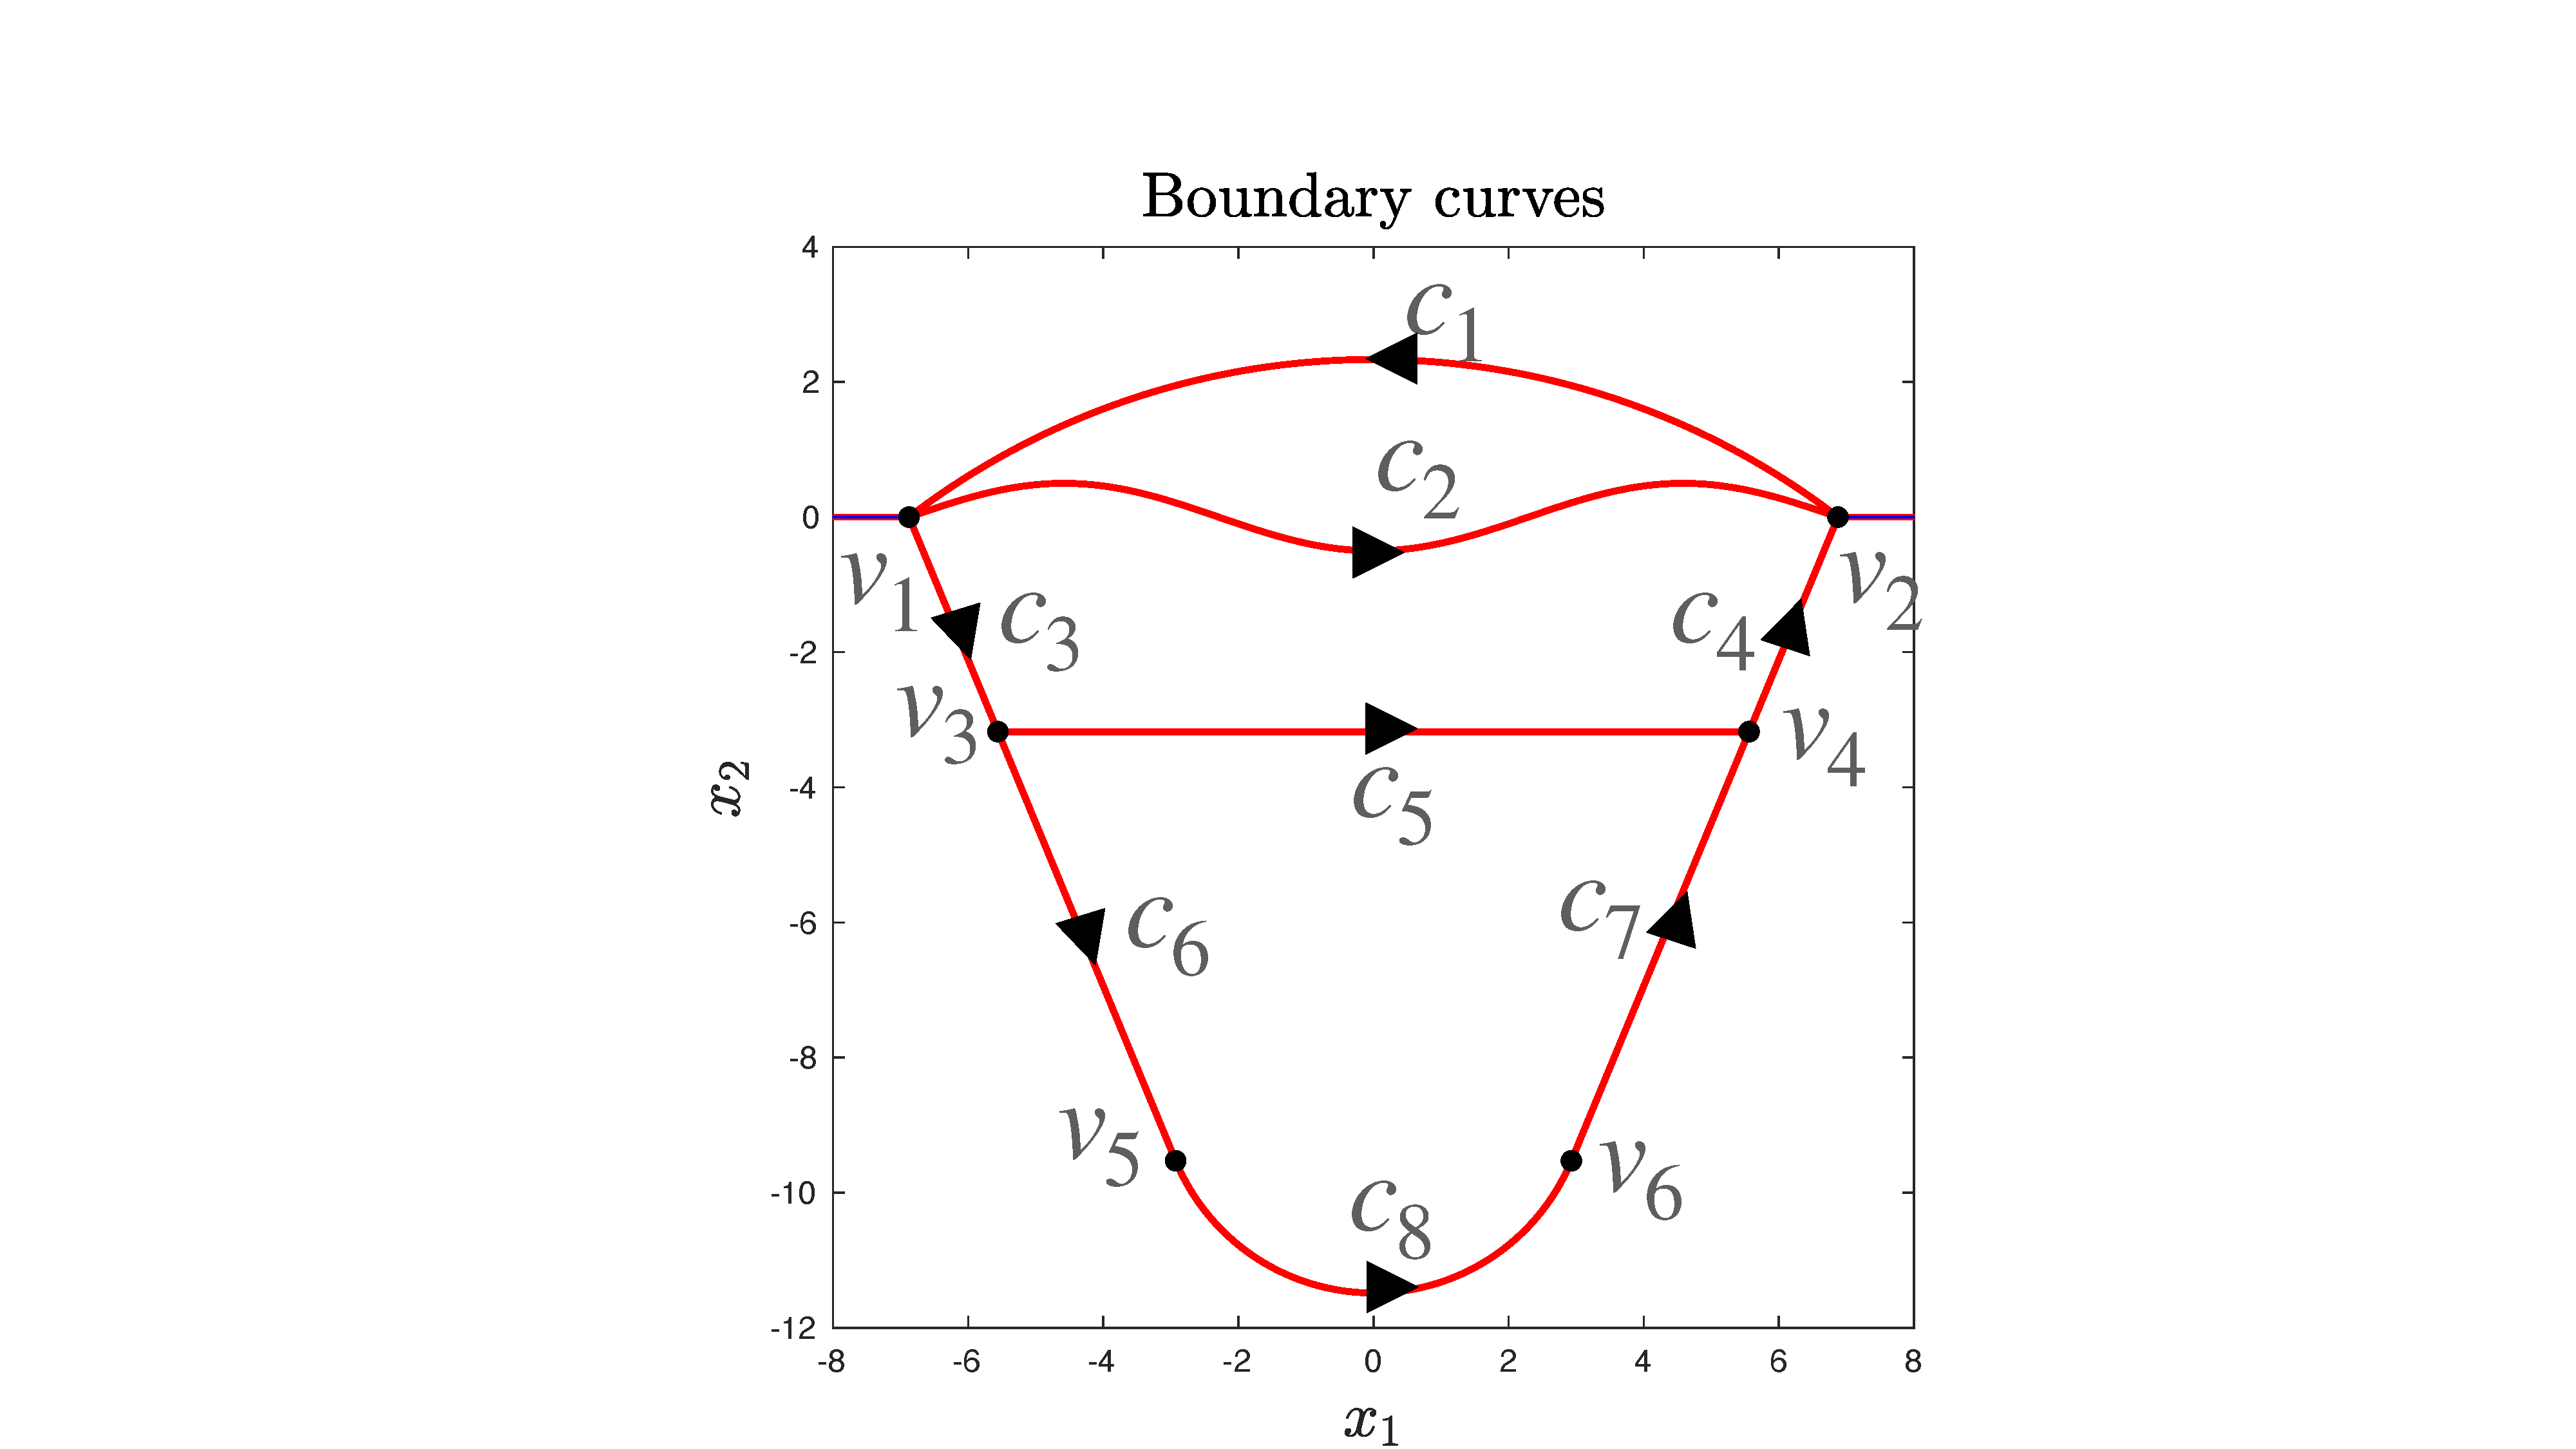
\includegraphics[width=0.5\linewidth]{example_geom}
\caption{Example geometry in test1.h5 and test1.mat}
\end{center}
\label{fig:1}
\end{figure}


For the group or cell \texttt{curves}, the attributes or variables are given by:
\begin{itemize}
\item Group $/\texttt{curves}/1$ or \texttt{curves\{1\}}
\begin{itemize}
\item \texttt{curvetype} = 2
\item \texttt{curve\_id} = 1
\item \texttt{vert\_list} = $[1,2]$
\item \texttt{ifconvex} = 0
\item \texttt{theta} = $\pi/2.4$
\end{itemize}
\item Group $/\texttt{curves}/2$ or \texttt{curves\{2\}}
\begin{itemize}
\item \texttt{curvetype} = 3
\item \texttt{curve\_id} = 2
\item \texttt{vert\_list} = $[1,2]$
\item \texttt{nwiggles} = 3
\item \texttt{amplitude} = $0.5$
\end{itemize}
\item Group $/\texttt{curves}/3$ or \texttt{curves\{3\}}
\begin{itemize}
\item \texttt{curvetype} = 1
\item \texttt{curve\_id} = 3
\item \texttt{vert\_list} = $[1,3]$
\end{itemize}
\item Group $/\texttt{curves}/4$ or \texttt{curves\{4\}}
\begin{itemize}
\item \texttt{curvetype} = 1
\item \texttt{curve\_id} = 4
\item \texttt{vert\_list} = $[4,2]$
\end{itemize}

\item Group $/\texttt{curves}/5$ or \texttt{curves\{5\}}
\begin{itemize}
\item \texttt{curvetype} = 1
\item \texttt{curve\_id} = 5
\item \texttt{vert\_list} = $[3,4]$
\end{itemize}

\item Group $/\texttt{curves}/6$ or \texttt{curves\{6\}}
\begin{itemize}
\item \texttt{curvetype} = 1
\item \texttt{curve\_id} = 6
\item \texttt{vert\_list} = $[3,5]$
\end{itemize}

\item Group $/\texttt{curves}/7$ or \texttt{curves\{7\}}
\begin{itemize}
\item \texttt{curvetype} = 1
\item \texttt{curve\_id} = 7
\item \texttt{vert\_list} = $[6,4]$
\end{itemize}

\item Group $/\texttt{curves}/8$ or \texttt{curves\{8\}}
\begin{itemize}
\item \texttt{curvetype} = 2
\item \texttt{curve\_id} = 8
\item \texttt{vert\_list} = $[5,6]$
\item \texttt{ifconvex} = 1
\item \texttt{theta} = $3\pi/4$
\end{itemize}
\end{itemize}


For the group or cell \texttt{regions}, the attributes or variables are given by:
\begin{itemize}
\item Group $/\texttt{regions}/1$ or \texttt{regions\{1\}}
\begin{itemize}
\item \texttt{region\_id} = 1
\item \texttt{icurve\_list} = $[-1]$
\item \texttt{is\_inf} = 1
\end{itemize}

\item Group $/\texttt{regions}/2$ or \texttt{regions\{2\}}
\begin{itemize}
\item \texttt{region\_id} = 2
\item \texttt{icurve\_list} = $[-4,-7,-8,-6,-3]$
\item \texttt{is\_inf} = -1
\end{itemize}


\item Group $/\texttt{regions}/3$ or \texttt{regions\{3\}}
\begin{itemize}
\item \texttt{region\_id} = 3
\item \texttt{icurve\_list} = $[1,2]$
\item \texttt{is\_inf} = 0
\end{itemize}


\item Group $/\texttt{regions}/4$ or \texttt{regions\{4\}}
\begin{itemize}
\item \texttt{region\_id} = 4
\item \texttt{icurve\_list} = $[-2,3,5,4]$
\item \texttt{is\_inf} = 0
\end{itemize}


\item Group $/\texttt{regions}/5$ or \texttt{regions\{5\}}
\begin{itemize}
\item \texttt{region\_id} = 5
\item \texttt{icurve\_list} = $[-5,6,8,7]$
\item \texttt{is\_inf} = 0
\end{itemize}

\end{itemize}


\end{document}  
